\documentclass{book}

\PassOptionsToPackage{unicode,pdfusetitle}{hyperref}
\PassOptionsToPackage{hyphens}{url}
\PassOptionsToPackage{dvipsnames,svgnames,x11names}{xcolor}

% Small caps serif font, for Paper numbers, ISBN, etc
\newcommand{\I}{\textrm{\scshape i}\xspace}
\newcommand{\II}{\textrm{\scshape ii}\xspace}
\newcommand{\III}{\textrm{\scshape iii}\xspace}
\newcommand{\IV}{\textrm{\scshape iv}\xspace}
\newcommand{\V}{\textrm{\scshape v}\xspace}
\newcommand{\VI}{\textrm{\scshape vi}\xspace}
\newcommand{\VII}{\textrm{\scshape vii}\xspace}
\newcommand{\VIII}{\textrm{\scshape viii}\xspace}
\newcommand{\IX}{\textrm{\scshape ix}\xspace}
\newcommand{\X}{\textrm{\scshape x}\xspace}
\newcommand{\ISBN}{\textrm{\scshape isbn}\xspace}
\newcommand{\ISSN}{\textrm{\scshape issn}\xspace}

\usepackage{pageslts}

% G5 format
\usepackage[
  paperwidth=169mm,
  paperheight=239mm,
  nomarginpar,
]{geometry}

\usepackage[T1]{fontenc}
\usepackage{mathtools}
\usepackage[varqu,varl,scale=0.93]{inconsolata}
\usepackage[ebgaramond,textscale=0,semibold,vvarbb,amsthm]{newtx}
\usepackage[scale=0.9]{cabin}
\usepackage{bm}

\usepackage{pifont} % for dingbats

\usepackage{upquote} % straight quotes in verbatim environments
\usepackage{microtype}
\UseMicrotypeSet[protrusion]{basicmath} % disable protrusion for tt fonts

% Additional font sizes \HUGE and \ssmall, needed for figure captions
\usepackage{moresize}

% tikz and pgfplots
\usepackage{tikz}
\usetikzlibrary{calc,arrows,shapes,positioning,intersections}
\usepackage{pgfplots}
\usepgfplotslibrary{external,colormaps}
\pgfplotsset{compat=1.11}
\tikzexternalize[export=false]

\usepackage[labelfont=bf]{caption}
\usepackage[labelfont=bf]{subcaption}

\usepackage{epigraph}

% algorithms
\usepackage[ruled,vlined,linesnumbered]{algorithm2e}
% \usepackage{algpseudocode,algorithm}
% \resetcounteronoverlays{algocf}

\usepackage{xcolor}
\usepackage{xurl}
\usepackage{bookmark}
\usepackage{hyperref}

\definecolor{lublue}{RGB}{0,0,128}
\definecolor{lubronze}{RGB}{156,97,20}

\hypersetup{
  colorlinks = true,
  % hidelinks,
  breaklinks = true,
  linkcolor  = lublue,
  filecolor  = lublue,
  urlcolor   = lublue,
  citecolor  = lubronze
}
\usepackage{cleveref}

% Chapters should have numbers - a typical thesis consists of two chapters:
% One to introduce and summarize the research ("kappa"), and one for
% reproductions of the papers and manuscripts. No need to number them by default.
% If you need chapter numbers back, comment the following line.
\renewcommand{\thesection}{\arabic{section}}

% Sections and subsections have numbers, subsubsections etc do not.
% \setcounter{secnumdepth}{2}

% Only chapters and sections appear in the table of contents, not subsections etc
\addtocontents{toc}{\protect\setcounter{tocdepth}{1}}

% Ensures that \cleardoublepage inserts empty pages without page number
\usepackage{emptypage}

% For text macros (e.g., small caps macros)
\usepackage{xspace}

% For "Lorem Ipsum" style place holders
\usepackage{blindtext}

% For \includegraphics
\usepackage{graphicx}

% Nice looking tables with correct spacings 
\usepackage{booktabs}
\usepackage{multirow}

% Tables spanning more than one page
% \usepackage{longtable}

% Math symbols
% \usepackage{amsfonts,amsmath,amssymb}

% To include the PDFs of the papers
\usepackage[]{pdfpages}

% Hyphenation, support for different languages, last one is default
% Make sure to install the hyphenation packages for all languages you need
\usepackage[english]{babel}

% Figures can be kept in the same directory as the thesis, or in a Figure/
% directory, without need to specifying which of the two it is
\graphicspath{{figures/}}

%%%%%%%%%%%%%%%%%%%%%%%%%%%%%%%%%%%%%%%%%%%%%%%%%%%%%%%%%%%%%%%%%%%%
% define commands for chapters, sections, and subsections that do not
% have a number, but are entered as candidates for the table of contents.

\newcommand\chap[1]{%
  \chapter*{#1}%
  \addcontentsline{toc}{chapter}{#1}
  \markboth{#1}{#1}
}
\newcommand\sect[1]{%
  \section*{#1}%
  \addcontentsline{toc}{section}{#1}
  \markright{#1}
}
\newcommand\subsect[1]{%
  \subsection*{#1}%
  \addcontentsline{toc}{subsection}{#1}
}

% References should be a section of the summary text, with number and all ...
% \renewcommand\bibsection{\section{\bibname}\markright{\bibname}}

% code listings
\usepackage{listings}

% Define a custom color
\definecolor{backcolour}{rgb}{0.95,0.95,0.95}
\definecolor{codegreen}{rgb}{0,0.6,0}
\definecolor{mygray}{rgb}{0.6,0.6,0.6}

\lstdefinestyle{myStyle}{
  backgroundcolor=\color{backcolour},
  frame=single,
  % commentstyle=\color{codegreen},
  basicstyle=\ttfamily\small,
  breakatwhitespace=false,
  breaklines=true,
  keepspaces=true,
  numbers=left,
  % numbersep=5pt,
  numberstyle=\footnotesize\color{mygray},
  showspaces=false,
  showstringspaces=false,
  showtabs=false,
  tabsize=2,
}

% Use \lstset to make myStyle the global default
\lstset{style=myStyle}

\usepackage{enumitem}

\usepackage{siunitx}

\usepackage[
  style=authoryear-comp,
  language=english,
  url=false,
  sortcites=true,
  refsegment=chapter,
  % minbibnames=22,
  % mincitenames=22,
  % maxbibnames=22,
  % maxcitenames=25
]{biblatex}
\addbibresource{phdthesis.bib}

% Problem environment
\usepackage{aliascnt}
\newaliascnt{problem}{equation}
\aliascntresetthe{problem}
\creflabelformat{problem}{#2\textup{(#1)}#3}
\makeatletter
\def\problem{$$\refstepcounter{problem}}
\def\endproblem{\eqno \hbox{\@eqnnum}$$\@ignoretrue}
\makeatother
\Crefname{problem}{Problem}{Problems}

\usepackage{fancyhdr}
\renewcommand{\chaptermark}[1]{\markboth{#1}{}}
\renewcommand{\sectionmark}[1]{\markright{#1}}
\pagestyle{fancy}
\fancyhf{}
\fancyhead[LE,RO]{\thepage}
\fancyhead[LO]{\itshape\scshape\nouppercase{\rightmark}}
\fancyhead[RE]{\itshape\nouppercase{\leftmark}}
\renewcommand{\headrulewidth}{0pt}

% operators
\DeclareMathOperator*{\argmax}{arg\,max}
\DeclareMathOperator*{\argmin}{arg\,min}
\DeclareMathOperator{\E}{E}
\DeclareMathOperator{\var}{Var}
\DeclareMathOperator{\cov}{Cov}
\DeclareMathOperator{\tr}{tr}
\DeclareMathOperator{\diag}{diag}
\DeclareMathOperator{\proj}{proj}
\DeclareMathOperator{\prox}{prox}
\DeclareMathOperator{\range}{range}
\DeclareMathOperator{\nullspace}{null}
\DeclareMathOperator{\rank}{rank}
\DeclareMathOperator{\card}{card}
\DeclareMathOperator{\sign}{sign}
\DeclareMathOperator{\st}{S}
\DeclareMathOperator{\normal}{Normal}
\DeclareMathOperator{\fnormal}{FoldedNormal}
\DeclareMathOperator{\bernoulli}{Bernoulli}
\DeclareMathOperator{\erf}{erf}
\DeclareMathOperator{\mse}{MSE}
\DeclareMathOperator{\risk}{R}
% \DeclareMathOperator{\I}{I}
% \DeclareMathOperator{\T}{}
%
% \DeclareMathSymbol{\phi}{\mathalpha}{operators}{0}
\DeclareMathOperator{\pdf}{\phi}
\DeclareMathOperator{\cdf}{\Phi}
% commands
% \newcommand{\vec}{\vectorsym}
% \newcommand{\mat}{\matrixsym}
\renewcommand{\vec}{\boldsymbol}
\newcommand{\mat}{\boldsymbol}
\newcommand*\du{\mathop{}\!\mathrm{d}}
% \newcommand{\T}{\mathsf{T}}
\newcommand{\T}{\intercal}
\newcommand{\ones}{\boldsymbol{1}}
\newcommand{\zeros}{\boldsymbol{0}}
% \newcommand{\T}{\intercal}
% \newcommand{\T}[1]{{1}^{\mathsf{T}}}
\newcommand{\ind}[1]{\operatorname{I}_{#1}}

% environments
\theoremstyle{plain}
\newtheorem{theorem}{Theorem}[section]
\newtheorem{corollary}{Corollary}[theorem]
\newtheorem{lemma}{Lemma}[section]
\newtheorem{proposition}{Proposition}[section]

\theoremstyle{definition}
\newtheorem{definition}{Definition}[section]
\newtheorem{example}{Example}[section]

\theoremstyle{remark}
\newtheorem{remark}[theorem]{Remark}

\newcommand{\todojl}[1]{\todo[color=green!40]{#1}}

\newcommand{\mv}[1]{{\boldsymbol{\mathrm{#1}}}}

\newcommand{\pkg}[1]{\texttt{#1}}
\newcommand{\lang}[1]{\texttt{#1}}
\newcommand{\data}[1]{\texttt{#1}}

% \newcommand{\iterate}{\textcolor{black}{\ding{108}}}
\newcommand{\textiterate}{\ding{108}}
\newcommand{\optimum}{\textcolor{orange}{\ding{54}}}

\newcommand{\bvec}{\vec{\beta}}
\newcommand{\bscal}{\beta}

\newcommand{\papertitle}[1]{{\bfseries #1}}
\newcommand{\paperauthors}[1]{{#1}}
\newcommand{\paperref}[1]{{#1}}
\newcommand{\papersep}{\\[0.5mm]}
\newcommand{\authorsep}{\\[1mm]}
\newcommand{\isbn}[1]{{\scshape isbn:~#1}}
\newcommand{\publication}[1]{{\itshape #1}}
% \newcommand{\refsep}{\\[3mm]}


% Re-usable information (title page, datasheet)
\newcommand{\myName}{Johan Larsson}
\newcommand{\myYear}{2024}
\newcommand{\myMainTitle}{Optimization and Algorithms in Sparse Regression}
\newcommand{\mySubTitle}{Screening Rules, Coordinate Descent, and Normalization}

% Compact combination of combining title and subtitle, used in datasheet and as
% chapter title for the main part.
\newcommand{\myTitle}{\myMainTitle: \mySubTitle}

\newcommand{\myFaculty}{Lund University School of Economics and Business Administration}
\newcommand{\myDepartment}{Department of Statistics}
\newcommand{\myAddress}{Box 7080\\SE--220 07 Lund\\Sweden} % Three lines maximum!

\newcommand{\myDegree}{Thesis for the degree of Doctor of Philosophy}
\newcommand{\myAdvisors}{Jonas Wallin and Małgorzata Bogdan}
\newcommand{\myOpponent}{Professor Mário A. T. Figueiredo (Instituto Superior Técnico, Lisbon, Portugal)}

\newcommand{\myDefenceAnnouncement}{%
  To be presented, with the permission of the
  \myFaculty\xspace of Lund University, for public criticism in the Clark Kent
  lecture hall (Kentsalen) at the \myDepartment\xspace
  on Sunday, the 34th of December \myYear\xspace at 24:00. }
\newcommand{\myCoverFront}{%
  \noindent {\bf Cover illustration front:}
  The elastic net path for a data set of diabetes patients.
}
\newcommand{\myCoverBack}{%
  {\bf Cover illustration back:} Picture showing my research (Paper \V).}
\newcommand{\myFundingInformation}{%
  {\bf Funding information:}
  The thesis work was financially supported by my rich uncle.}

% \newcommand{\mySeries}{\ISSN: $<$ISSN number$>$}

\newcommand{\myISBNprint}{978-91-8104-076-0}
\newcommand{\myISBNpdf}{978-91-8104-077-7}
\newcommand{\myFormSignDate}{1776-7-4}

% total page number is computed automatically:
\newcommand{\myPages}{\lastpageref{LastPages}}

\newcommand{\myFormDefenceDate}{2024-05-24}
\newcommand{\myFormKeywords}{%
  power, victory, awesomeness}

% Write a short english abstract of the thesis here, goes into the data sheet page 4. 
\newcommand{\myAbstract}{
  \blindtext

  \blindtext
}%

% --- Shortcut thesis commands for paper references and titles ---
% Included papers - only need to type this once
\newcommand{\PaperIauthor}{\textbf{F. Lastname}, C. Coauthor, \ldots}
\newcommand{\PaperIIauthor}{\textbf{F. Lastname}, C. Coauthor, \ldots}
\newcommand{\PaperIIIauthor}{\textbf{F. Lastname}, C. Coauthor, \ldots}
\newcommand{\PaperIVauthor}{\textbf{F. Lastname}, C. Coauthor, \ldots}
\newcommand{\PaperVauthor}{\textbf{F. Lastname}, C. Coauthor, \ldots}
\newcommand{\PaperVIauthor}{\textbf{F. Lastname}, C. Coauthor, \ldots}

\newcommand{\PaperIref}{Journal for Superheroes, pp. 1--10}
\newcommand{\PaperIIref}{Journal for Bankers, pp. 2--30}
\newcommand{\PaperIIIref}{Journal for Superheroes, pp. 1--10}
\newcommand{\PaperIVref}{Journal for Superheroes, pp. 1--10}
\newcommand{\PaperVref}{Journal for Superheroes, pp. 1--10}
\newcommand{\PaperVIref}{Journal for Superheroes, pp. 1--10}

\newcommand{\PaperItitle}{The Strong Screening Rule for SLOPE}
\newcommand{\PaperIItitle}{Look-Ahead Screening Rules for the Lasso}
\newcommand{\PaperIIItitle}{The Hessian Screening Rule}
\newcommand{\PaperIVtitle}{Benchopt: Reproducible, Efficient and Collaborative Optimization Benchmarks}
\newcommand{\PaperVtitle}{Coordinate Descent for SLOPE}
\newcommand{\PaperVItitle}{Regularization and Scaling in Sparse Regression}

\makeatletter
\newcommand*{\rom}[1]{\expandafter\scshape\romannumeral #1}
\makeatother

\newcommand{\PaperSeparator}[1]{%
  \begin{tikzpicture}[remember picture, overlay]
    \node[
      fill=black,
      text=white,
      font=\bfseries\fontsize{50}{55}\selectfont,
      anchor=east,
      minimum height=1.5cm,
      minimum width=2.6cm,
      text width=2.0cm,
      align=left
      ] at ($(current page.north east) + (0,-{#1*0.15}\paperheight + 0.75cm)$)  {\rom{#1}};
  \end{tikzpicture}
}

% Not included papers, in case you want to list them
%\newcommand{\PaperNotIncIauthor}{C. Coauthor, \textbf{X. Someone}}
%\newcommand{\PaperNotIncIref}{Journal for \ldots}
%\newcommand{\PaperNotIncItitle}{Boring matter}
% --- END reusable thesis commands ---

\begin{document}

%%%%%%%%%%%%% First pages with thesis title etc %%%%%%%%%%%%%%%%%%%%%%%%%%%%%%%%
% First six pages are contained in a separate file. Normally you should not
% need to edit it.

\pagestyle{empty}

% This file contains the layout of the first six pages and the explanation text
% of a compilation thesis. 

%%%%%%%%%%%%% FIRST PAGES WITH THESIS TITLE ETC %%%%%%%%%%%%%%%%%%%%%%%%%%%%%%%%
\frontmatter % roman numbers

% Page one: Title only
\thispagestyle{empty} % no page number
\begin{center}
  \vspace*{5cm}
  {\Large \myMainTitle}
  %\\
  %{\large \mySubTitle}
\end{center}

% Page two: empty. Empty space is important

%%%%%%%%%%%%%%%%%%%%%%%%%%%%%%%%%%%%%%%%%%%%%%%%%%%%%%%%%%%%%%%%%%%%%%%
% Page three: title page with small text (spikningsblad)

\cleardoublepage
\thispagestyle{empty} % no page number
~
\vfill
\begin{center}
  {\HUGE \myMainTitle}
  \\[2mm]
  {\huge \mySubTitle}

  \vfill
  {\myName}

  \vfill
  % black and white (default):
  
\includegraphics[width=0.25\textwidth]{LundUniversity_C2line_BLACK.eps}

  \vspace{10mm}
  {\large \myDegree}\\
  {\large Thesis advisors: \myAdvisors}\\
  {\large Faculty opponent: \myOpponent}\\
  \vspace{1cm}
  {\footnotesize
    \myDefenceAnnouncement
  }
  \\
\end{center}
\vfill

%%%%%%%%%%%%%%%%%%%%%%%%%%%%%%%%%%%%%%%%%%%%%%%%%%%%%%%%%%%%%%%%%%%%%%%
% Page four: data sheet
\newpage

%Either include datasheet texfile (will be filled in automatically), or a pdf
%containing datasheet (text needs to be already in it, edit
%sheetPDF_editable.pdf). Use one of the next two lines: 
\newcounter{aformdx}
\newcounter{aformdy}
\newcounter{aformx}
\newcounter{aformy}
\newcounter{aformtx}
\newcounter{aformtdx}
\newcounter{aformty}
\def\aformw{358}
\def\aformwhalf{\aformw / 2}
\def\aformwquart{\aformw / 4}
\def\aformwthreeq{\aformw / 4 * 3}
\def\aformh{517}
\def\aformb{23}
\def\aformlinew{0.4pt}
\def\aformrowh{20}
\def\aformRowh{24}
\newcommand\aformhline
{\put(\value{aformx},\value{aformy}){\line(1,0){\value{aformdx}}}}
\newcommand\aformvline
{\put(\value{aformx},\value{aformy}){\line(0,-1){\value{aformdy}}}}
\newcommand\aformvlinec
{\put(\value{aformx},\value{aformy}){\line(0,-1){16.25}}}
\newcommand\aformboxbase[5]
{
  \setcounter{aformtx}{\value{aformx}}
  \setcounter{aformtdx}{\value{aformdx}}
  \setcounter{aformty}{\value{aformy}}
  \addtocounter{aformtx}{#1}
  \addtocounter{aformtdx}{-#2}
  \addtocounter{aformty}{-#3}
  \put(\value{aformtx},\value{aformty})
  {
    \parbox[t]{\value{aformtdx}pt}
    {{\sf\tiny #4}{\scriptsize #5\par}}
  }
}
\newcommand\aformbox[2]{\aformboxbase{2}{11}{8}{#1}{#2}}
\newcommand\aformBox[2]{\aformboxbase{2}{11}{8}{#1}{#2}}

\begin{center}
  \begin{picture}(\aformw,510)(0,0)
    \linethickness{\aformlinew}
    \put(0,\aformb){\framebox(\aformw,\aformh){}}
    \put(-14,200){\rotatebox{90}{\parbox{200pt}
        {\sf\tiny
          DOKUMENTDATABLAD
          enl SIS 61 41 21\\
        }}}
    \setcounter{aformx}{0}
    \setcounter{aformy}{\aformb}
    \addtocounter{aformy}{\aformh}
    \setcounter{aformdx}{\aformwhalf}
    \aformbox{Organization}
    {\\
    {\bf LUND UNIVERSITY}\vspace{0.1cm}
    \\
    {\myDepartment\\
    \myAddress}
    }
    \setcounter{aformdy}{\aformrowh}
    \addtocounter{aformdy}{\aformrowh}
    \addtocounter{aformdy}{\aformrowh}
    \addtocounter{aformdy}{\aformRowh}
    \setcounter{aformx}{\aformwhalf}
    \aformvline
    \setcounter{aformx}{0}
    \addtocounter{aformy}{-\aformrowh}
    \addtocounter{aformy}{-\aformrowh}
    \addtocounter{aformy}{-\aformRowh}
    \aformbox{Author(s)}{\\\myName}
    \setcounter{aformdy}{\aformrowh}
    \aformhline
    \addtocounter{aformy}{\aformrowh}
    \addtocounter{aformy}{\aformrowh}
    \addtocounter{aformy}{\aformRowh}
    \setcounter{aformx}{\aformwhalf}
    \aformbox{Document name}{\\{\bf DOCTORAL DISSERTATION}}
    \addtocounter{aformy}{-\aformrowh}
    \aformhline
    \aformbox{Date of disputation}{\\\myFormDefenceDate}
    \setcounter{aformx}{\aformwhalf}
    \aformhline
    \addtocounter{aformy}{-\aformrowh}
    \addtocounter{aformdy}{\aformRowh}
    \aformbox{Sponsoring organization}{}
    \aformhline
    \addtocounter{aformy}{-\aformRowh}
    \addtocounter{aformy}{-\aformrowh}
    \setcounter{aformx}{0}
    \setcounter{aformdx}{\aformw}
    \aformhline
    \aformbox{Title and subtitle }{\\\myTitle}
    \addtocounter{aformy}{-\aformRowh}
    \setcounter{aformx}{0}
    \aformhline
    \aformBox{Abstract}
    {\\
    {\parskip0pt\parindent1em
    \myAbstract
    }
    }
    \setcounter{aformy}{\aformb}
    % Correspond to one minus each in the bottom section
    \addtocounter{aformy}{\aformRowh}
    \addtocounter{aformy}{\aformRowh}
    \addtocounter{aformy}{\aformRowh}
    \addtocounter{aformy}{\aformRowh}
    \addtocounter{aformy}{\aformrowh}
    \addtocounter{aformy}{\aformrowh}
    \addtocounter{aformy}{10}
    \addtocounter{aformy}{10}
    \aformhline
    \aformbox{Key words}
    {
      \\\myFormKeywords
    }
    \addtocounter{aformy}{-\aformRowh}
    \addtocounter{aformy}{-10}
    \aformhline
    \aformbox{Classification system and/or index terms (if any)}{}
    \addtocounter{aformy}{-\aformRowh}
    \aformhline
    \aformbox{Supplementary bibliographical information}{}
    \setcounter{aformx}{\aformwthreeq}
    \setcounter{aformdx}{\aformwquart}
    \setcounter{aformdy}{\aformRowh}
    \aformvline
    \aformbox{Language}{\\English}
    \addtocounter{aformy}{-\aformRowh}
    \setcounter{aformx}{0}
    \setcounter{aformdx}{\aformw}
    \aformhline
    \aformbox{ISSN and key title}{}
    \setcounter{aformx}{\aformwthreeq}
    \addtocounter{aformdy}{10}
    \aformvline
    \addtocounter{aformdy}{-10}
    \aformbox{ISBN}{\\\myISBNprint\xspace(print)\\\myISBNpdf\xspace(pdf)}
    \addtocounter{aformy}{-\aformRowh}
    \addtocounter{aformy}{-10}
    \setcounter{aformx}{0}
    \aformhline
    \aformbox{Recipient's notes}{}
    \setcounter{aformx}{\aformwhalf}
    \setcounter{aformdy}{\aformrowh}
    \addtocounter{aformdy}{\aformrowh}
    \aformvline
    \aformbox{Number of pages}{\\227}
    \setcounter{aformx}{\aformwthreeq}
    \aformbox{Price}{}
    \setcounter{aformdy}{\aformrowh}
    \aformvline
    \addtocounter{aformy}{-\aformrowh}
    \setcounter{aformx}{\aformwhalf}
    \setcounter{aformdx}{\aformwhalf}
    \aformhline
    \aformbox{Security classification}{}
    \setcounter{aformx}{0}
    \setcounter{aformdx}{\aformw}
    \addtocounter{aformy}{-\aformrowh}
    \addtocounter{aformy}{-4}
    \aformbox{}
    {\scriptsize I, the undersigned, being the copyright owner of the abstract of the
      above-mentioned dissertation, hereby grant to all reference sources
      the permission to publish and disseminate the abstract of the
      above-mentioned dissertation.
    }
    \addtocounter{aformy}{-\aformRowh}
    \addtocounter{aformy}{-20}
    \aformbox{
      \hspace{0pt}
      %\put(44,1){\includegraphics{images/signature}} %Media-Tryck does not want this to be included as a graphic
    }{}
    \aformbox{\rm
      \scriptsize
      Signature \underline{\hskip 140pt}\hfill Date \underline{\hskip 80pt}
    }{}
    \addtocounter{aformy}{1}
    \aformbox{}{\hskip 280pt \scriptsize \myFormSignDate}
  \end{picture}
\end{center}

%\addtocounter{pages}{1} 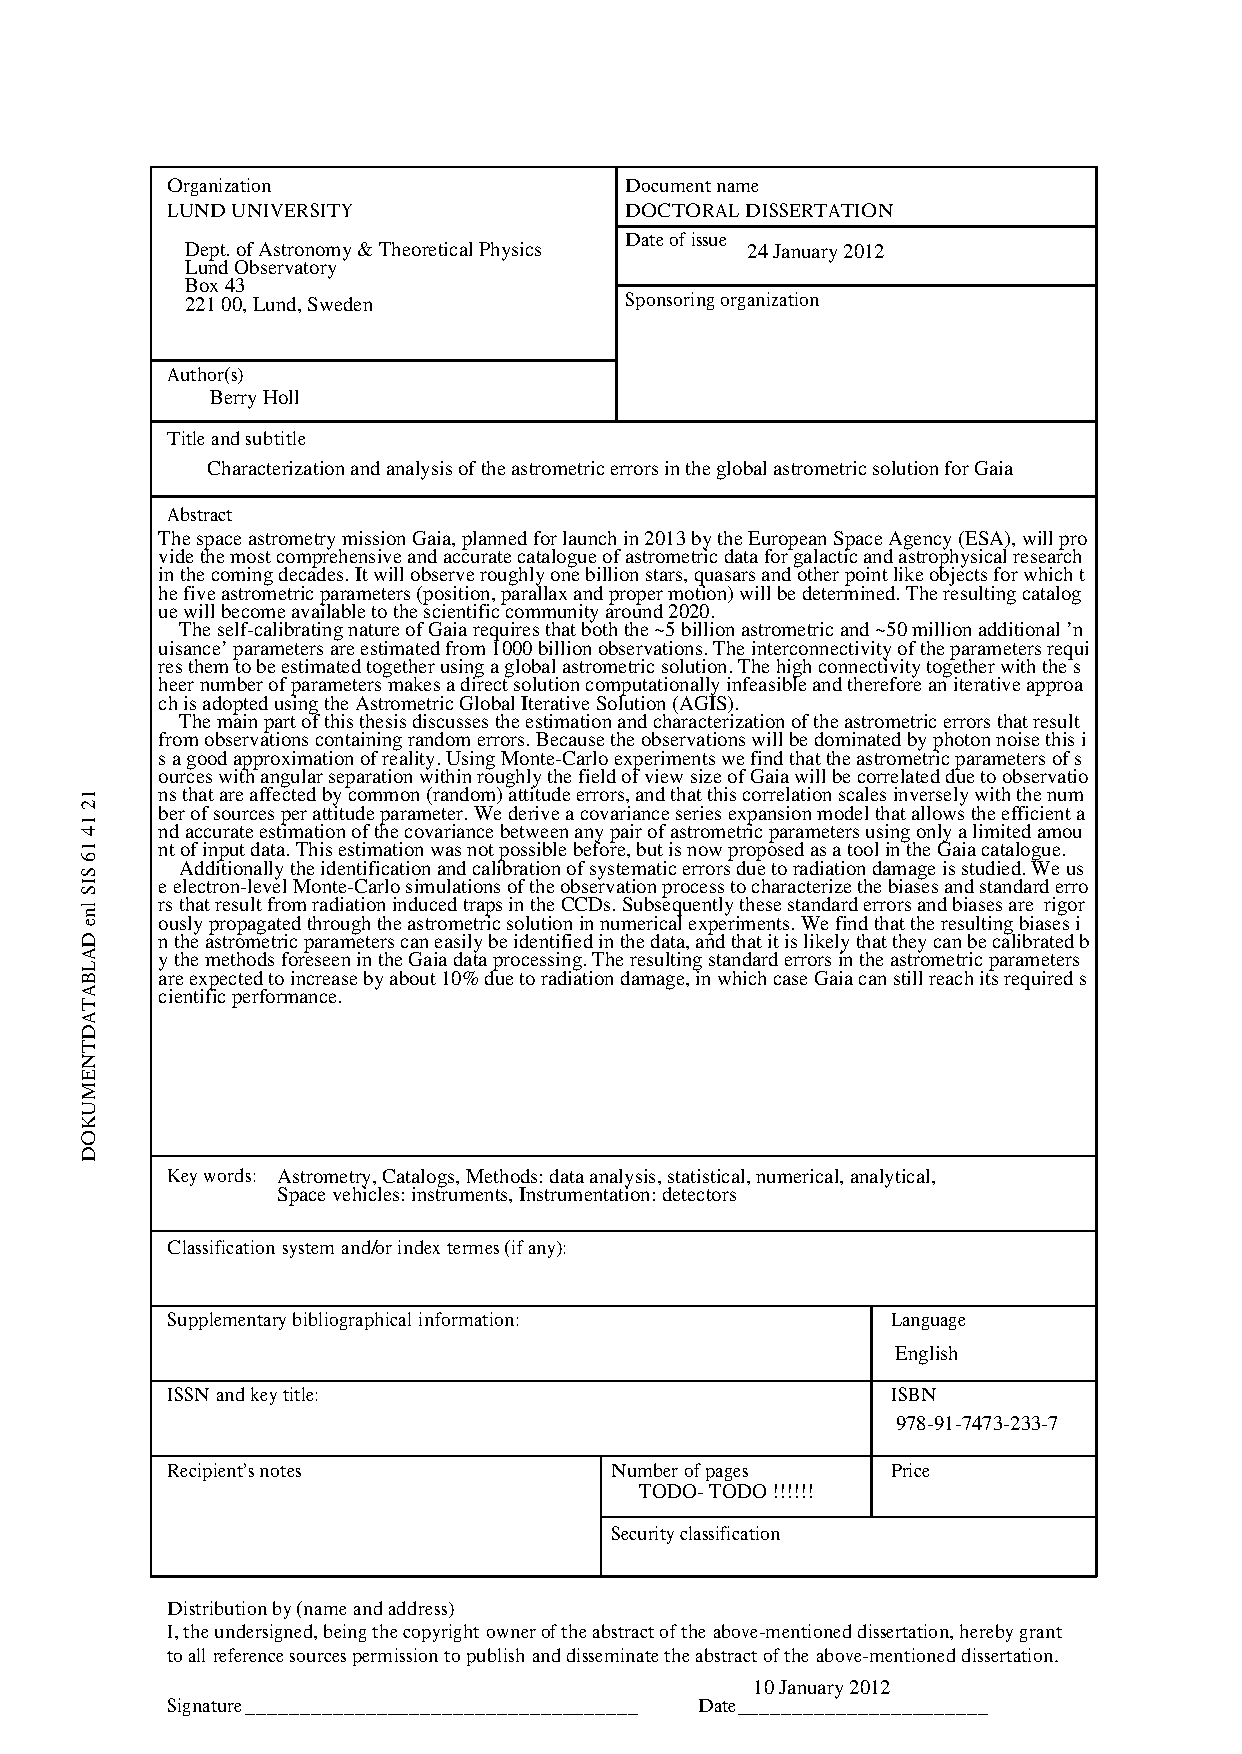
\includepdf[pages=1-1]{datasheetPDF_editable}

%%%%%%%%%%%%%%%%%%%%%%%%%%%%%%%%%%%%%%%%%%%%%%%%%%%%%%%%%%%%%%%%%%%%%%%
% Page five: title and author, without small text. Looks good!

\cleardoublepage
\thispagestyle{empty} % no page number
~
\vfill
\begin{center}
  {\HUGE \myMainTitle}
  \\[2mm]
  {\huge \mySubTitle}

  \vfill
  {\myName}

  \vfill
  % black and white (default):
  
\includegraphics[width=0.25\textwidth]{LundUniversity_C2line_BLACK.eps}

  % Colour text in white so that the spacing is the same as on page three, but with less clutter
  \color{white}{
  \vspace{10mm}
  {\large \myDegree}\\
  {\large Thesis advisors: \myAdvisors}\\
  {\large Faculty opponent: \myOpponent}\\
  \vspace{1cm}
  {\footnotesize
    \myDefenceAnnouncement
  }
  }
  \\
\end{center}
\vfill


%%%%%%%%%%%%%%%%%%%%%%%%%%%%%%%%%%%%%%%%%%%%%%%%%%%%%%%%%%%%%%%%%%%%%%%
% Page six: Cover image description, ISBN, copyright
\newpage

\thispagestyle{empty} % no page number

\noindent A doctoral thesis at a university in Sweden takes either the form of a single,
cohesive research study (monograph) or a summary of research papers
(compilation thesis), which the doctoral student has written alone or together
with one or several other author(s).

In the latter case the thesis consists of two parts. An introductory text puts
the research work into context and summarizes the main points of the papers.
Then, the research publications themselves are reproduced, together
with a description of the individual contributions of the authors. The
research papers may either have been already published or are manuscripts at
various stages (in press, submitted, or in draft).

\vfill
{\small
  \myCoverFront\\
  \\
  \myCoverBack\\
  \\
  \myFundingInformation


  \vspace{5mm}
  \noindent\copyright\, \myName~\myYear\\
  \\
  \myFaculty, {\myDepartment}
  \\
  \\
  \ISBN: \myISBNprint~(print)\\ % ISBN av svenska ISBN centralen
  \ISBN: \myISBNpdf~(pdf)\\ % ISBN av svenska ISBN centralen
  \mySeries\\
  \\
  Printed in Sweden by Media-Tryck, Lund~University, Lund~\myYear

  \medskip

  \noindent
\includegraphics[width=0.5\textwidth]{ENG-Miljologotyper-sid-2-BLACK.eps}
}


% Quote page

\newpage
\thispagestyle{empty} % No page number on quote page

\setlength\epigraphrule{0pt}
\setlength\epigraphwidth{.5\textwidth}

\null
\vspace{20ex}

% Nothing in life is as important as you think it is when you are thinking about it. ---Daniel Kahneman
% Our comforting conviction that the world makes sense rests on a secure foundation: our almost unlimited ability to ignore our ignorance.
% As you know from teaching introductory statistics, 30 is infinity. -- Andrew Gelman
% You should inform your gut and then trust it ---Daniel Kahneman
% The best thing about being a statistician is that you get to play in everyone's backyard. --- John Tukey

% \epigraph{\itshape
%   As you know from teaching introductory statistics, 30 is infinity.
% }{
%   ---Andrew Gelman
% }

\epigraph{\itshape
  There’s a point when you go with what you’ve got. Or you don’t go.
}{
  ---Joan Didion
}






\cleardoublepage

\pagestyle{headings}

% Table of Contents
\setcounter{page}{1} % Page Roman 1 of the frontmatter
\setcounter{tocdepth}{1}

\tableofcontents
\addtocontents{toc}{\protect\thispagestyle{empty}}

%%%%%%%%%%%%%%%%%%%%%%%%%%%%%%%%%%%%%%%%%%%%%%%%%%%%%%%%%%%%%%%%%%%%
%%%%%%%%%%% List of publications %%%%%%%%%%%%%%%%%%%%%%%%%%%
% Have a long list and want to start on the left page? Here, have a special
% chapter heading for that!
%\addcontentsline{toc}{part}{Part 1: Summary}
%\renewcommand{\chapterheadstartvskip}{}
%{\let\cleardoublepage\relax \let\chapterheadstartvskip\nop 

\newpage

\chap{Acknowledgements}

\newpage

\chap{Abstract}

\chap{Popular Science Summary}

\chap{List of Publications}\label{sec:paperlist}

This thesis is based on the following publications.

\begin{description}[leftmargin=!,labelwidth=0.7cm]
  \item[\I] \fullcite{larsson2020b}
  \item[\II] \fullcite{larsson2021}
  \item[\III] \fullcite{larsson2022b}
  \item[\IV] \fullcite{moreau2022a}
  \item[\V] \fullcite{larsson2023}
  \item[\VI] PAPER ON THE WAY
        % TODO: Add details for last paper
\end{description}

%   % Publications not included in this thesis:
%   % \vspace{2mm}
%   %
%   % \begin{tabularx}{\textwidth}{rX}
%   % {\sc \phantom{vi}}   & {\bf \PaperNotIncItitle}\\[2mm]
%   %	  & \PaperNotIncIauthor\\
%   %          & \PaperNotIncIref\\[5mm] 
%   %
%   %\end{tabularx}
%   %
% } % End large font tables, continue with font size stated in preamble

\noindent {\small All papers are reproduced with permission of their respective publishers.}

% Page numbers arabic 
\mainmatter
% Reset table counters to not count the publications table
\setcounter{table}{0}
% Rest page counters, this is where it all starts!
\setcounter{page}{1}

\chap{Introduction}
% Fancy a quote?
\begin{flushright}
  \textit{Everything should be made as simple as possible, but not simpler.}\\
  {---Albert Einstein}
\end{flushright}

\section{Background}

% With modern advances in science and technology, statistical models and the data on which they are fit are becoming increasingly complex. In many disciplines, such as bioinformatics, it is common to measure observations across many more variables than was previously the case. And so data sets are growing in size and becoming ever more high-dimensional. In some fields, this growth in complexity has been paralleled with more effective methods with which to collect observations, as in, for instance, the field of crowd science. But in other areas this this is still a costly endeavor. In bioinformatics, for example, ethical concerns and rising requirements on the quality of data have only raised the costs of data collection. As a result, the data collected in these fields is becoming \emph{wider}: the ratio between the number of variables and the number of observations is increasing. This has challenged classical statistical methods such as classical linear regression, which break down in this setting. And even if there are indeed methods that can be used to model such data, without reducing the number of parameters, the resulting models are often not interpretable. This is the problem that sparse regression methods attempt to solve.
%
% Sparse regression methods select only a subset of the features\footnote{A feature is the values of a variable or transformations of a variable for all the observations in the data. It is synonymous with \emph{predictor} and \emph{regressor}.} in the data set, setting the regression coefficients of the remaining ones to zero. The validity of doing so hinges on the assumption that the true model is in fact sparse, and this is called the \emph{sparsity assumption}, which can be motivated by the \emph{bet-on-sparsity principle}: Assume that the underlying model is sparse and use a sparse method to model it. If the assumption is correct, then our method has a chance of doing well. But if the assumption is incorrect, then our method will not work---but no other method would.
%
% The success of neural networks and other methods that model high-dimensional data well but do not enforce sparsity might seem to defy the validity of this principle. But this is not the case: if the true model truly is sparse, then we will always do better with a sparse method.
%
% Sparse regression methods have a long-standing history in statistics, starting in the 60's with the advent of stepwise regression methods, which are defined by their use of iterative procedures in which features are added or removed from a candidate model in steps. Typically, these algorithms use hypothesis tests to determine whether to add or remove a feature.
% The first popular stepwise method was invented by \textcite{efroymson1960}, which is a type of forward-stepwise algorithm. Efroymson's algorithm starts with an intercept-only model and then adds or removes features of the design matrix incrementally into the model. Later methods include backward-stepwise regression~\parencite{raiffa1968} and best-subset selection~\parencite{beale1967}, the latter considering all possible subsets of the features.
%
% Stepwise methods are now considered problematic for several reasons, such as yielding \(R^2\) values that are too high, \(p\)-values that are too small, and arbitrary variable selection when the variables are collinear\footnote{See \textcite[Chapter 4.3]{harrell2015} for a detailed discussion on this topic.}.
%
% Another important reason for why they are not used as much today is that they are computationally expensive since they need to consider all possible subsets of the features\footnote{\textcite{bertsimas2016} has recently shown that this might not be as much of a problem as previously thought. Apparently, the best-subset selection can be solved relatively efficiently using mixed-integer programming, which means that the problem is solvable in polynomial time.} This reason was part of the motivation for the development of regularized methods, which instead of solving standard regression problems on subsets of the features penalize the objective with a penalty that induces sparsity, and which can be fit using much more efficient methods. In this short report we will discuss these methods, the optimization algorithms underlying them, and their history. We will do so by focusing on two methods: the lasso and sorted \(\ell_1\) penalized estimation (SLOPE).

\section{Regularization}

For this thesis, we are in general interested in fitting regularized statistical models to tabular data consisting of a matrix of features (or predictors) \(\mat{X} \in \mathbb{R}^{n \times p}\) and a response vector \(\vec{y} \in \mathbb{R}^n\).

The models that we are interested in fitting are of the form

\begin{align*}
  \text{minimize} & f(\vec{\beta}; \mat{X}, \vec{y}) = g(\vec{\beta}; \mat{X}, \vec{y}) + h(\vec{\beta})
\end{align*}
where \(f(\beta)\)


\subsection{Lasso}

\subsection{Elastic Net}

\subsection{SLOPE}

\section{Optimization}

\section{Summary of the Papers}

\subsection{Paper \I}

In this paper, we address the challenge of extracting relevant features from data sets where the number of observations, n, is significantly smaller than the number of predictors, p. We focus on the Sorted L-One Penalized Estimation (SLOPE)—a generalization of the lasso—as a promising method in this context. However, current numerical procedures for SLOPE lack the efficiency that lasso tools possess, especially when estimating a complete regularization path. A key component of lasso's efficiency is predictor screening rules, which allow predictors to be discarded before model estimation. This paper is the first to establish such a rule for SLOPE. We develop a SLOPE screening rule by examining its subdifferential and demonstrate that this rule is a generalization of the strong rule for the lasso. Although our rule is heuristic and may occasionally discard predictors erroneously, we show that such instances are rare and can be easily safeguarded against by a simple check of the optimality conditions. Our numerical experiments reveal that the rule performs well in practice, leading to significant improvements for data in the \(p \gg n\) domain, and incurs no additional computational overhead when \(n > p\). This paper, therefore, presents a significant advancement in the efficiency of SLOPE, particularly in high-dimensional settings.

\subsection{Paper \II}

In this paper, we focus on the lasso, a widely used method for inducing shrinkage and sparsity in the solution vector of regression problems, especially when the number of predictors outweighs the number of observations. Solving the lasso in such high-dimensional settings can be computationally challenging. However, this challenge can be mitigated through the use of screening rules that discard predictors before fitting the model, resulting in a reduced problem. We introduce a new screening strategy, termed look-ahead screening. This method employs safe screening rules to identify a range of penalty values for which a specific predictor cannot enter the model, thereby screening predictors along the remaining path. Our experiments demonstrate that these look-ahead screening rules outperform the active warm-start version of the Gap Safe rules, marking a significant advancement in the efficiency of solving high-dimensional lasso problems.

\subsection{Paper \III}

In this paper, we address the challenge of predictor screening rules in l1-regularized regression problems, such as the lasso. These rules, which eliminate predictors from the design matrix before fitting a model, have significantly improved the speed of solving such problems. However, current state-of-the-art screening rules struggle with highly-correlated predictors, often becoming overly conservative. To tackle this issue, we introduce a new screening rule: the Hessian Screening Rule. This rule leverages second-order information from the model to provide more accurate screening and higher-quality warm starts. Our proposed rule outperforms all other alternatives we studied on datasets with high correlation for both l1-regularized least-squares (the lasso) and logistic regression. It also delivers the best performance overall on the real datasets we examined. This paper, therefore, presents a significant advancement in dealing with highly-correlated predictors in l1-regularized regression problems.

\subsection{Paper \IV}

In this paper, we tackle the challenges posed by the rapid development of machine learning research, particularly in the area of numerical validation. Researchers often face a multitude of methods to compare, lack of transparency and consensus on best practices, and the tedious task of re-implementing work. This often results in partial validation, which can lead to incorrect conclusions and hinder research progress. To address these issues, we introduce Benchopt, a collaborative framework designed to automate, reproduce, and publish optimization benchmarks in machine learning across different programming languages and hardware architectures. Benchopt simplifies the benchmarking process by providing a ready-to-use tool for running, sharing, and extending experiments. We demonstrate its wide applicability through benchmarks on three standard learning tasks: $\ell_2$-regularized logistic regression, Lasso, and ResNet18 training for image classification. These benchmarks reveal key practical findings that provide a more nuanced view of the state-of-the-art for these problems, emphasizing that the details matter in practical evaluation. We believe that Benchopt will encourage collaborative work in the community and improve the reproducibility of research findings.

\subsection{Paper \V}

In this paper we delve into the Sorted L-One Penalized Estimation (SLOPE), an extension of the renowned lasso regression method. Despite the promising statistical properties of SLOPE, its adoption has been limited due to the inefficiency of existing algorithms in high-dimensional contexts. To overcome this challenge, we introduce a novel, faster algorithm that solves the SLOPE optimization problem.

Our algorithm merges the techniques of proximal gradient descent and proximal coordinate descent, significantly enhancing the efficiency of the SLOPE method. We also shed new light on the directional derivative of the SLOPE penalty and its associated SLOPE thresholding operator, and provide assurances of convergence for our proposed solver. Through comprehensive benchmarks on both simulated and real data, we demonstrate that our method outperforms a host of competing algorithms. This paper is a significant contribution as it broadens the applicability of the SLOPE method in high-dimensional settings, potentially paving the way for its wider use in the field.

\subsection{Paper \VI}

In this paper, we explore the sensitivity of regularized methods, such as the lasso and ridge regression, to the scales of the features in the data. It's standard practice to normalize features to ensure they share the same scale. While standardization is common for continuous data, binary data, particularly when high-dimensional and sparse, is often not scaled at all. We demonstrate that this choice can significantly impact the estimated model when the binary features are imbalanced, and that these effects also depend on the type of regularization used. Specifically, we show that the size of a feature's corresponding coefficient in the lasso is directly related to its class imbalance, and this effect depends on the normalization used. We propose potential solutions to this issue and discuss the case when data is mixed, containing both continuous and binary features. This paper, therefore, provides valuable insights into the impact of feature scaling on regularized methods and offers practical solutions for handling mixed data.

\printbibliography

\chap{Papers}

\cleardoublepage

\thispagestyle{empty}

\phantomsection
\addcontentsline{toc}{section}{\protect\numberline{\I} {\PaperItitle}}
\markright{\I{}: \PaperItitle}

% \begin{tikzpicture}[remember picture, overlay]
%   \node[fill=black, text=white, font=\bfseries\fontsize{50}{55}\selectfont, anchor=east, minimum height=1.5cm, minimum width=2.5cm, text width=1.5cm, align=left] at ($(current page.north east) + (0,-0.2\paperheight)$) {\I};
% \end{tikzpicture}

\PaperSeparator{1}

\cleardoublepage
% Include the PDF. Comment this while writing the thesis, only add later.
% Options are: all pages, scaled to full width (use 0.95 if that is too high for some reason), with thesis page number
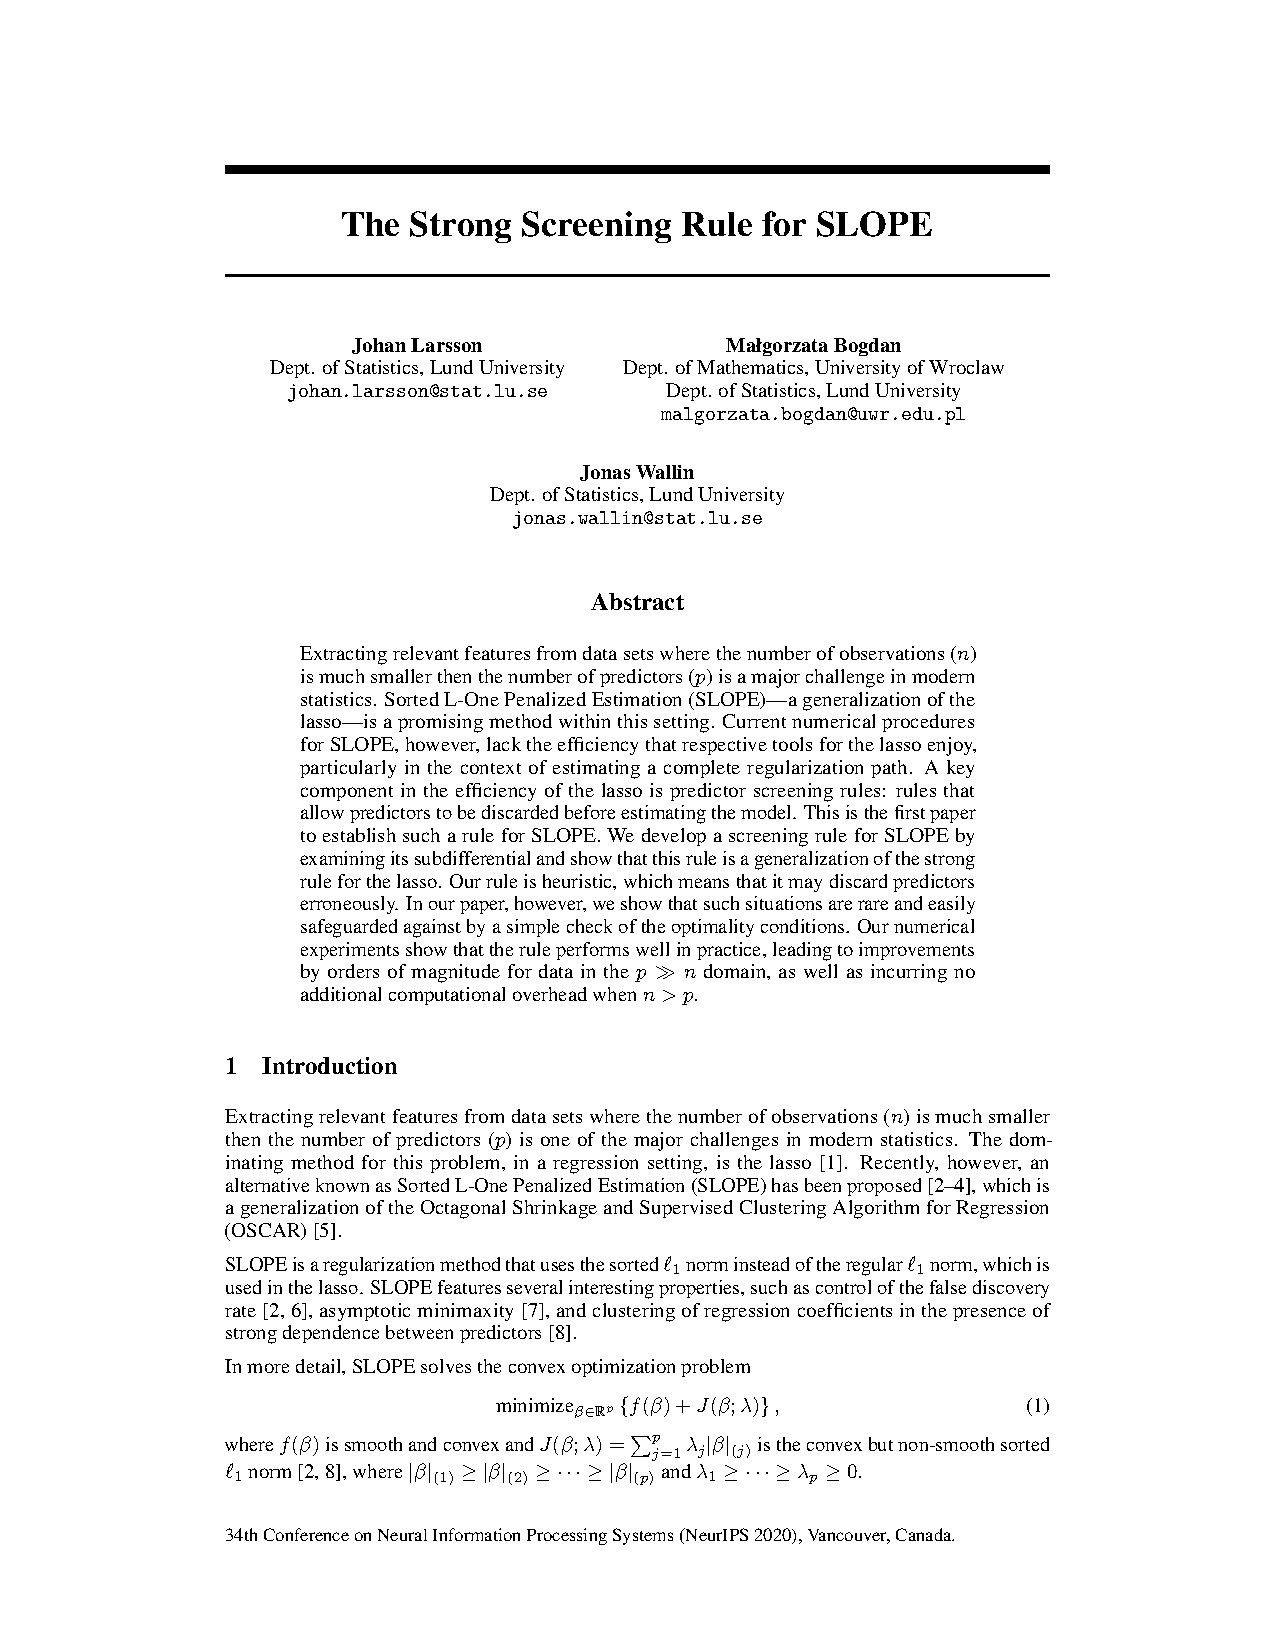
\includepdf[
  pages=-,
  width=0.9\textwidth,
  % scale=0.50,
  % noautoscale,
  % offset=-14.56723pt 0pt,
  % frame=true,
  clip,
  viewport=107 50 506 743,
  pagecommand={\thispagestyle{headings}},
]{papers/paper1.pdf}
% One additional option could be useful: To cut away the margins of the included PDFs use:
% clip,viewport=<left> <bottom> <right> <top>
% To determine the four numbers you can use the ./determineViewport.sh script in the thesis directory.

\cleardoublepage

\thispagestyle{empty}
\PaperSeparator{2}
\addcontentsline{toc}{section}{\protect\numberline{\II} {\PaperIItitle}}

\cleardoublepage

\thispagestyle{empty}
\PaperSeparator{3}
\addcontentsline{toc}{section}{\protect\numberline{\III} {\PaperIIItitle}}

\cleardoublepage

\thispagestyle{empty}
\PaperSeparator{4}
\addcontentsline{toc}{section}{\protect\numberline{\IV} {\PaperIVtitle}}

\cleardoublepage

\thispagestyle{empty}
\PaperSeparator{5}
\addcontentsline{toc}{section}{\protect\numberline{\V} {\PaperVtitle}}

\cleardoublepage

\thispagestyle{empty}
\PaperSeparator{6}
\addcontentsline{toc}{section}{\protect\numberline{\VI} {\PaperVItitle}}

\cleardoublepage

% \appendix
% \thispagestyle{empty}

% \begin{tikzpicture}[remember picture, overlay]
%   \node[fill=black, text=white, font=\bfseries\HUGE, anchor=east, minimum height=1.5cm, minimum width=5cm] at ($(current page.north east) + (0,-0.8\paperheight)$) {Appendix};
% \end{tikzpicture}

% \appendix
% \chap{Appendix: Conference posters}
% \section*{Poster 1: \PaperItitle}
% Media-Tryck's suggestion to a poster layout, can be downloaded from \url{https://bildweb.srv.lu.se/login/}.
% Presented 2067 at the \emph{Symposium for time travel}
% in Berlin, Germany. For further details refer to Paper~\I and
% Sect.~\ref{sec:mainresults}.
%
% % include poster itself. Cropping works as described above for the papers.
% 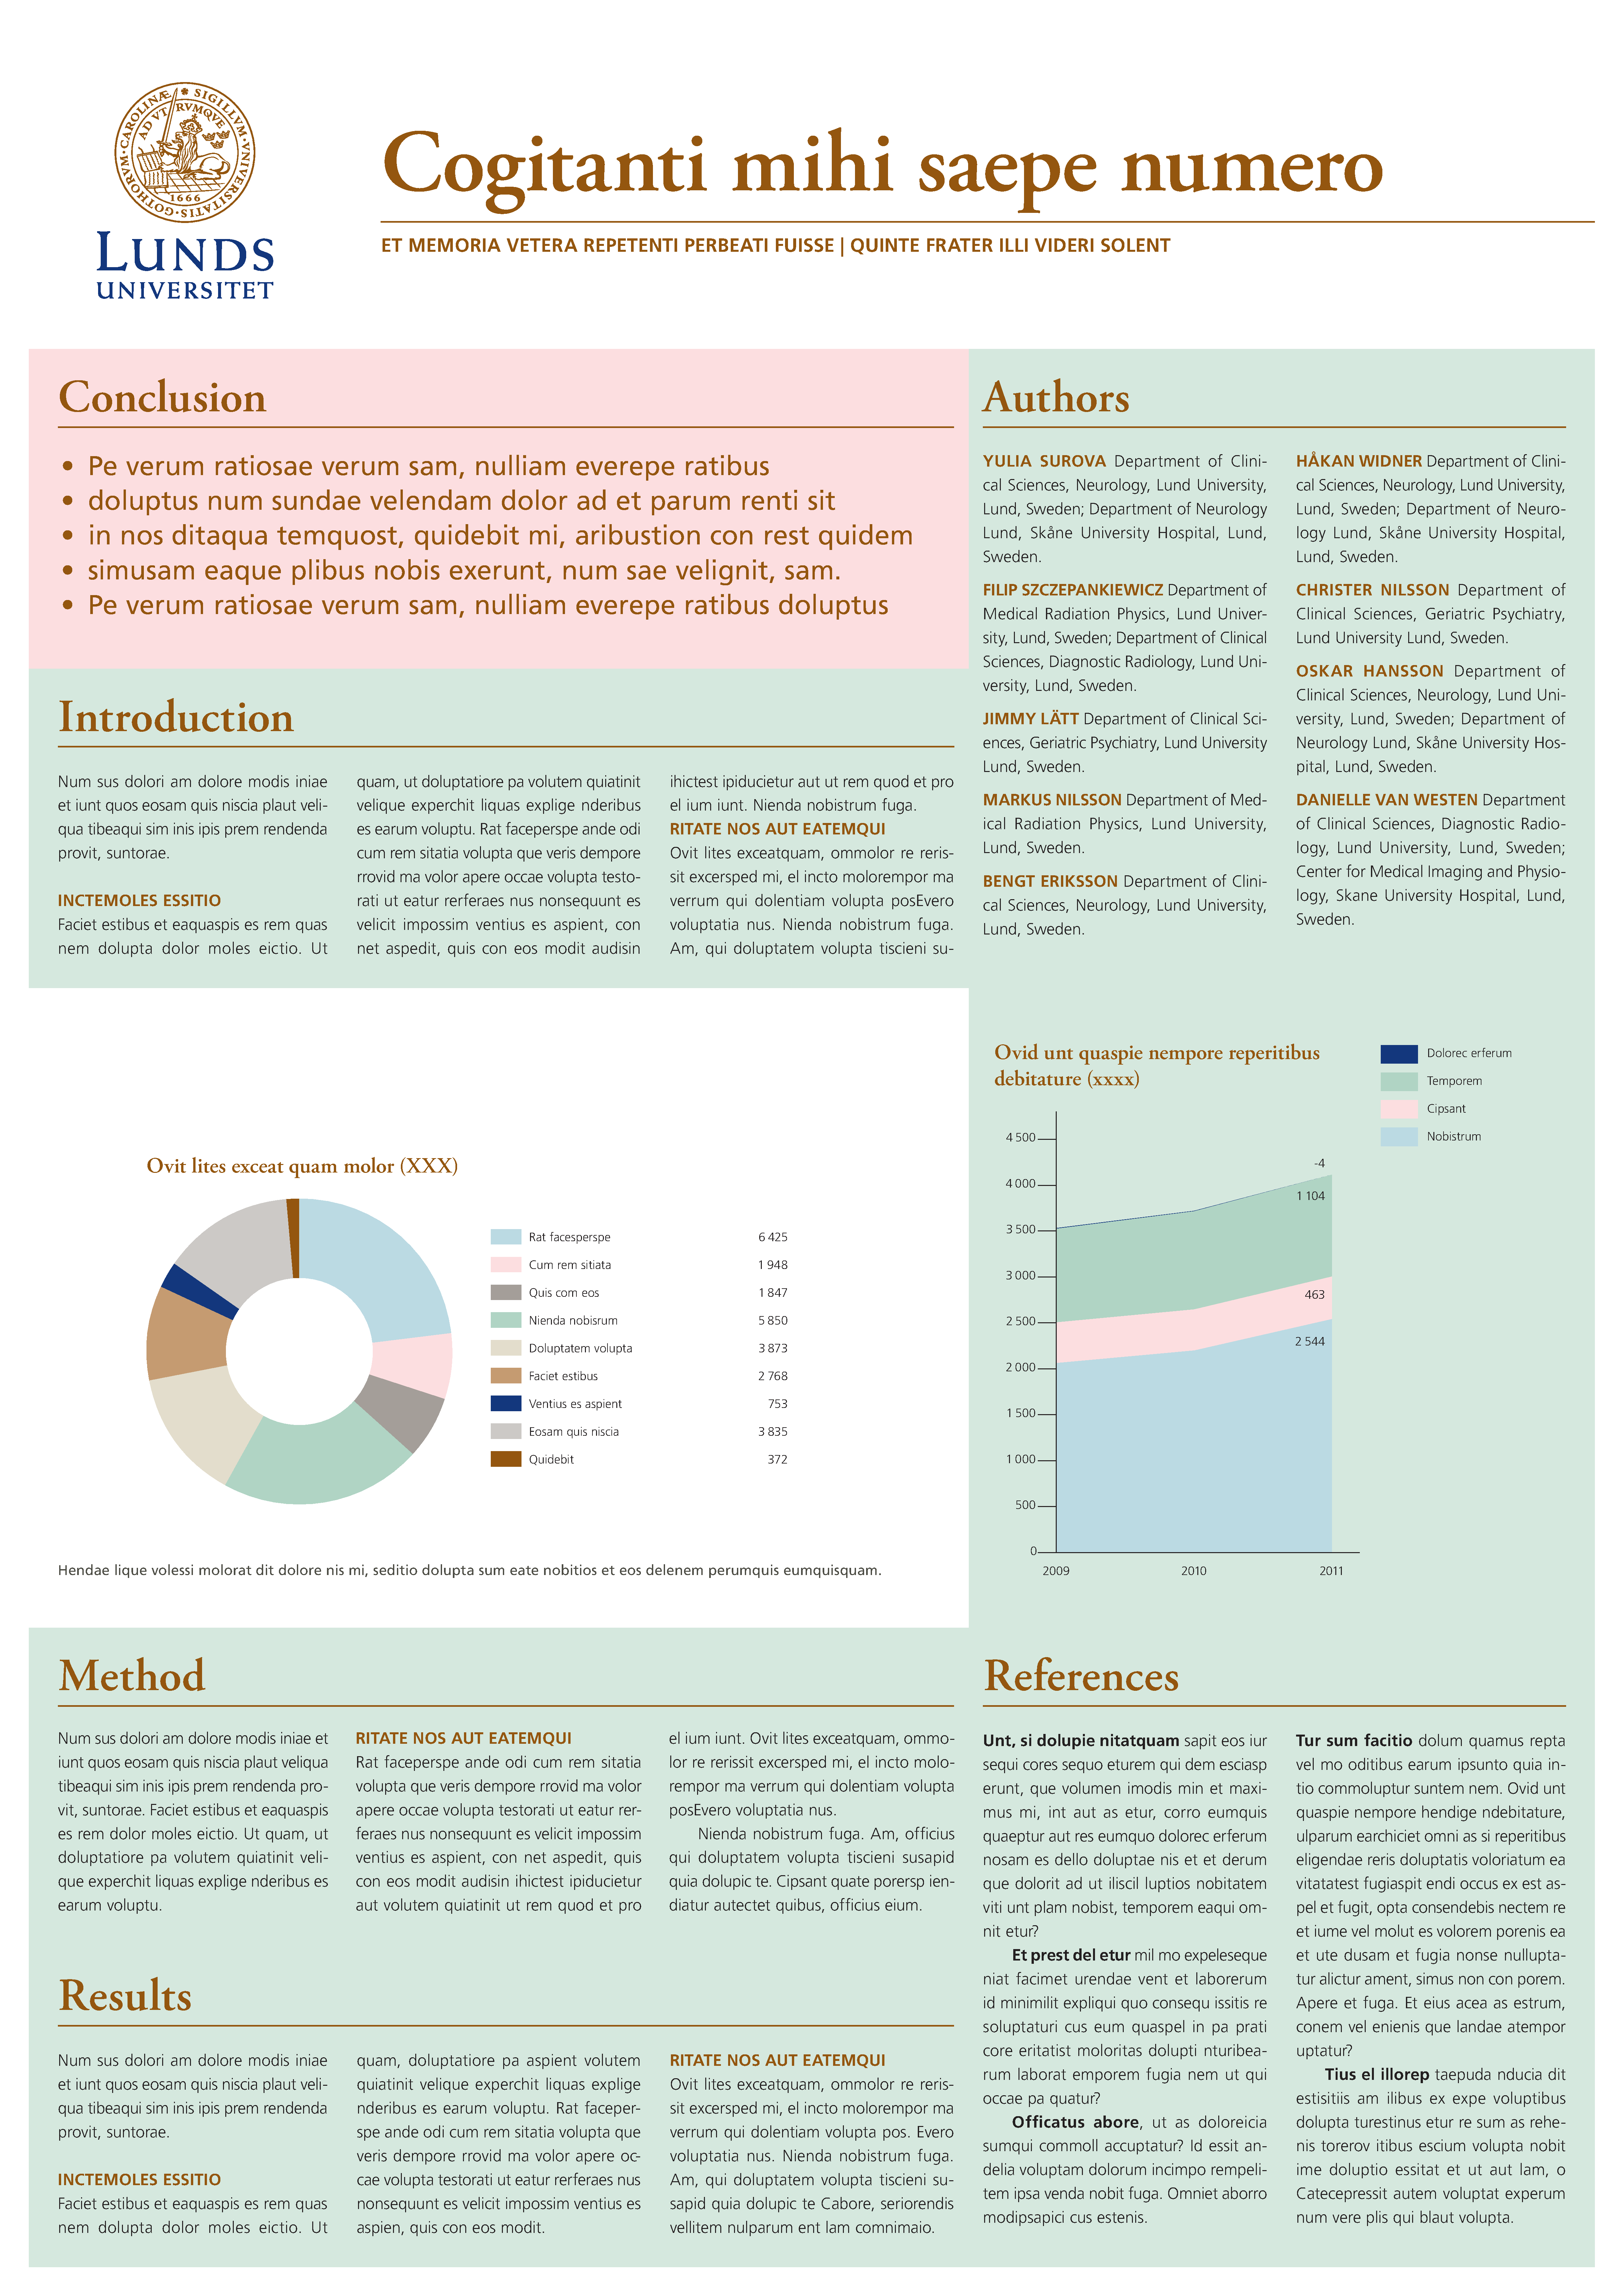
\includepdf[pages=-,width=\paperwidth-10mm]{posterMediaTryck.pdf} %smaller margin, works fine when printing (hopefully ;) Hallå, Jonas!)

\end{document}
